\chapter{功能仿真结果}

\section{利用Chisel3配套工具进行快速仿真}
Chisel3在Github网站上有一套基于Scala体系的仿真工具,chisel-testers。
使用该工具可以直接在Scala中实例化使用Chisel3开发的模块,并且产生激励进行模块的仿真。
其主要提供了一个名为PeekPokeTester的类,该类提供了能够完成激励产生和信号断言的方法。
\begin{table}[h] %开始一个表格environment,表格的位置是h,here。  
    \centering
    \caption{PeekPokeTester中提供的方法} %显示表格的标题  
    \begin{tabular}{l|l|c} %设置了每一列的宽度,强制转换。  
    \hline  
    \hline  
    方法名 & 作用 & 使用举例 \\ %用&来分隔单元格的内容 \\表示进入下一行  
    \hline %画一个横线,下面的就都是一样了,这里一共有4行内容  
    poke & 设置DUT的输入信号 & poke(c.io.in.valid, 1) \\
    \hline  
    peek & 读取DUT的输出信号 & peek(c.io.out.bits) \\
    \hline  
    expect & 比较DUT的输出信号 & expect(c.io.out.bit, 0xff) \\
    \hline  
    step & 驱动DUT的时钟信号 & step(1) \\
    \hline
    reset & 驱动DUT的复位信号 & reset(1) \\
    \hline  
    \hline  
    \end{tabular}  
\end{table}
同时,该工具支持使用Verilator作为仿真后端,大大降低了大规模电路的仿真时间,借助Verilator,可以产生仿真时的vcd仿真文件,通过GTKWave、Verdi等波形查看工具即可查看仿真波形,
使用时十分便利。相比于Verilog环境下编写行为复杂的testbench,Chisel-Tester提供的解决方案依赖于面向对象编程,逻辑更加清晰,不易出错。
            \begin{lstlisting}[title=Chisel Test Example, frame=shadowbox]
class Tester(c: Test) extends PeekPokeTester(c) {
  poke(c.io.in, -1)     //Set DUT input "in" as -1
  step(1)               //wait 1 clock
  expect(c.io.out, -1)  //assert DUT output "out" as -1
}
            \end{lstlisting}

\section{基于FIFO的可变长移位寄存器仿真结果}
% filters: DenseVector(0, 2, -1) __ 3
% filterNum: 1
% imgs: DenseVector(4, -3, -3, -1, -5) __ 5
% imgNum: 1
% nchannel: 1
\begin{figure}[h]
    \centering
    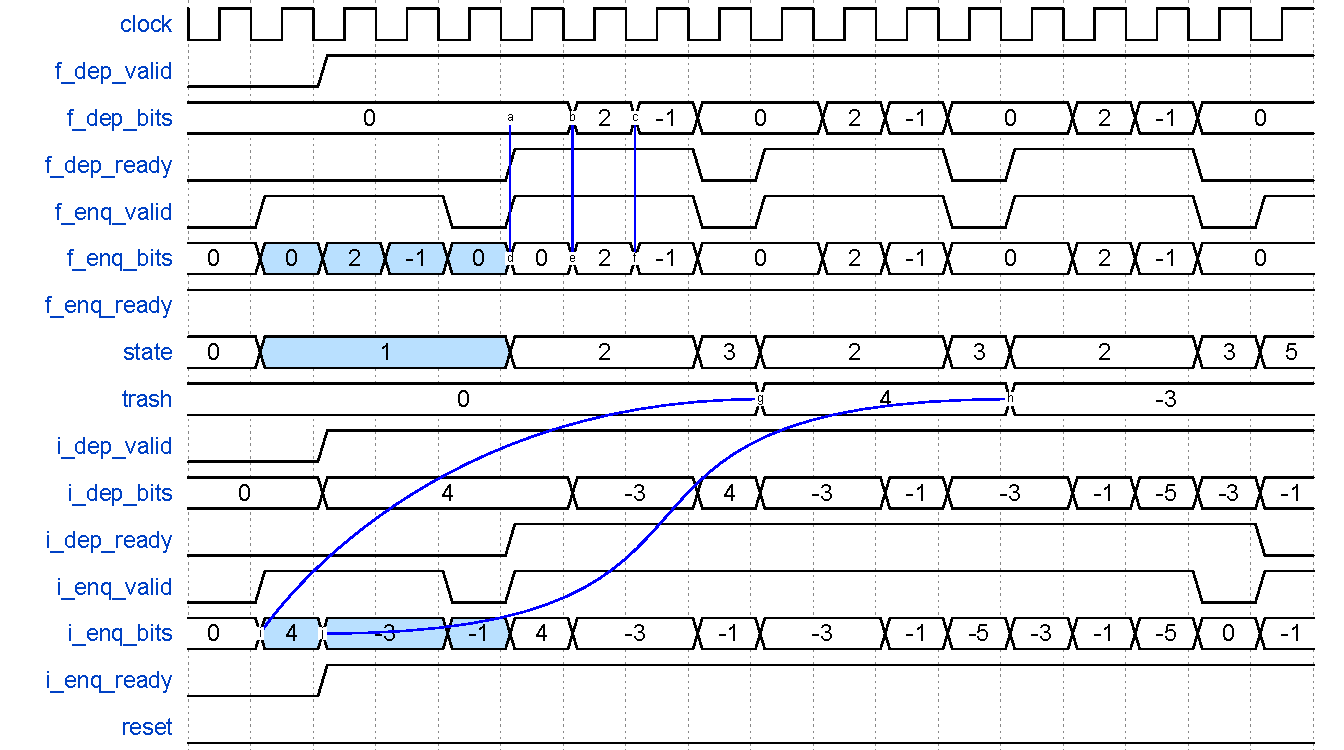
\includegraphics[scale=0.7]{../pdf/shift_w.pdf}\\
    \caption{基于FIFO的可变长移位寄存器仿真波形图}
    \label{shift_w}
\end{figure}
该模块的逻辑行为切换由\emph{state}信号控制。
当\emph{state=0}时该模块不工作,
\emph{state=1}时,模块内嵌的FIFO输入接口通过Mux与外部输入数据接口对接,此时开始存储外部数据,如图\ref{shift_w}阴影部分所示,此时filter FIFO中依次存入了0,-2,-1,img FIFO中依次存入了4,-3,-3。
\emph{state=2}时,模块内嵌FIFO输入接口通过Mux与自身的输出接口对接,形成环路,此时被弹出的数据再次回到FIFO中以完成循环移位寄存器的功能,如图\ref{shift_w},\emph{f\_dep}信号组中出现的连接线,弹出的0,2,-1同时又写回FIFO。
\emph{state=3}时,模块中FIFO数据已经全部计算完成,根据卷积计算的特性,此时需要弹出部分数据之后接受等长的新数据,由于FIFO输入接口与输出接口互不干扰,因此可以弹出废弃数据的同时接受新的数据,如图\ref{shift_w}\emph{i\_enq}和\emph{i\_deq}信号组中的连接线,最开始存入的4,-3分别在两次中弹出,同时两次中分别接受了-1,-5两个新数据。
\begin{figure}[h]
    \centering
    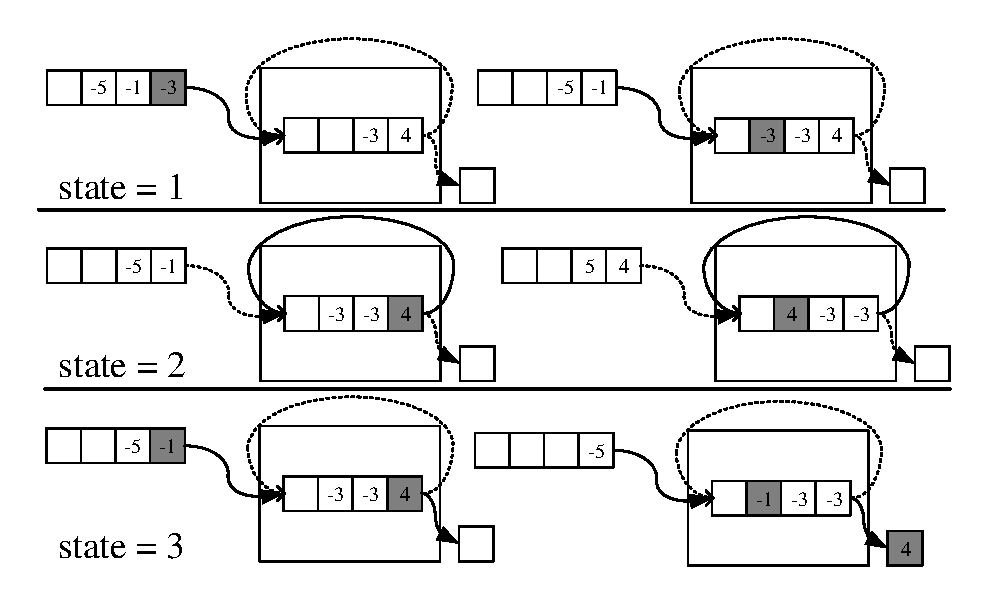
\includegraphics[scale=0.8]{../pdf/shift_k.pdf}\\
    \caption{基于FIFO的可变长移位寄存器工作示意图}
    \label{shift_k}
\end{figure}
该模块的工作示意图可以参考\ref{shift_k}。

\section{Designware SRAM IP仿真结果}
\begin{figure}[h]
    \centering
    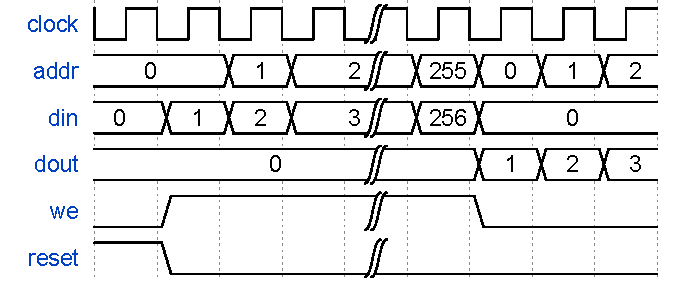
\includegraphics{../pdf/sram_w.pdf}\\
    \caption{SRAM IP波形图}
\end{figure}

\section{PE单元仿真结果}
$[4,-3,-3,-1,-5] * [0,2,-1]$
\begin{figure}[h]
    \centering
    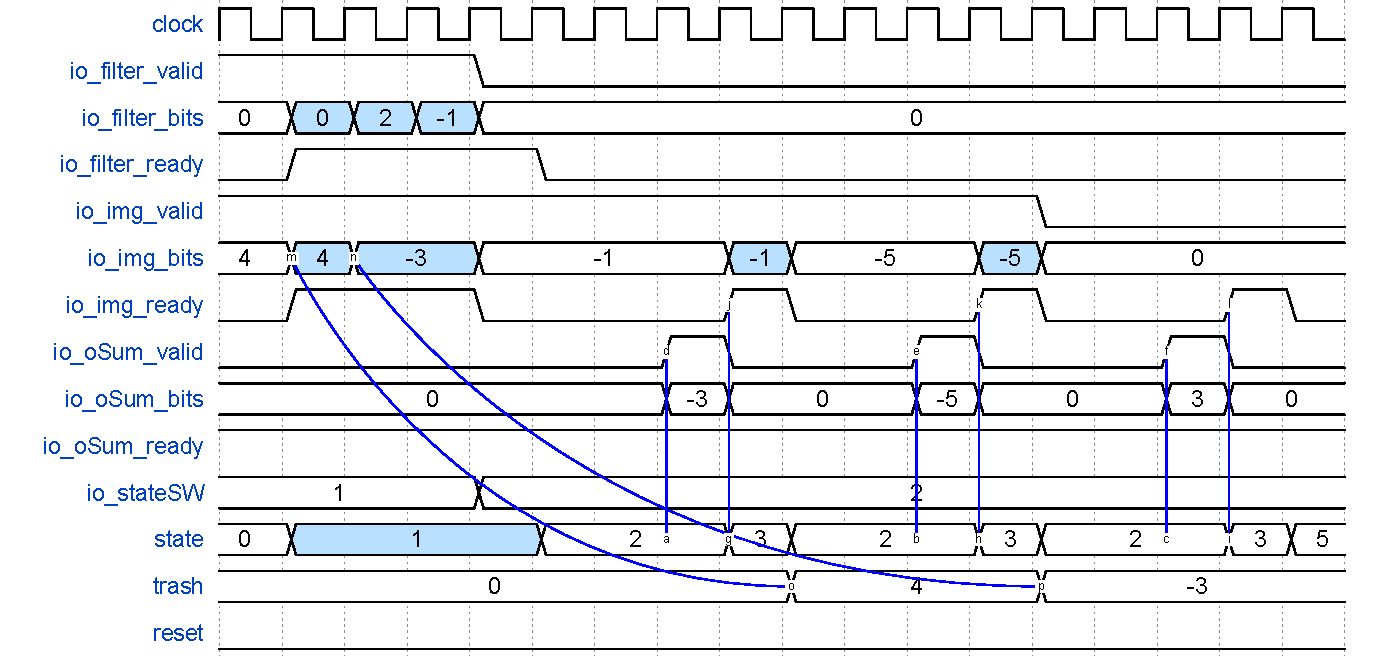
\includegraphics[scale=0.7]{../pdf/pe_w.pdf}\\
    \caption{PE波形图}
\end{figure}

\section{PE阵列仿真结果}
\begin{figure}[h]
    \centering
    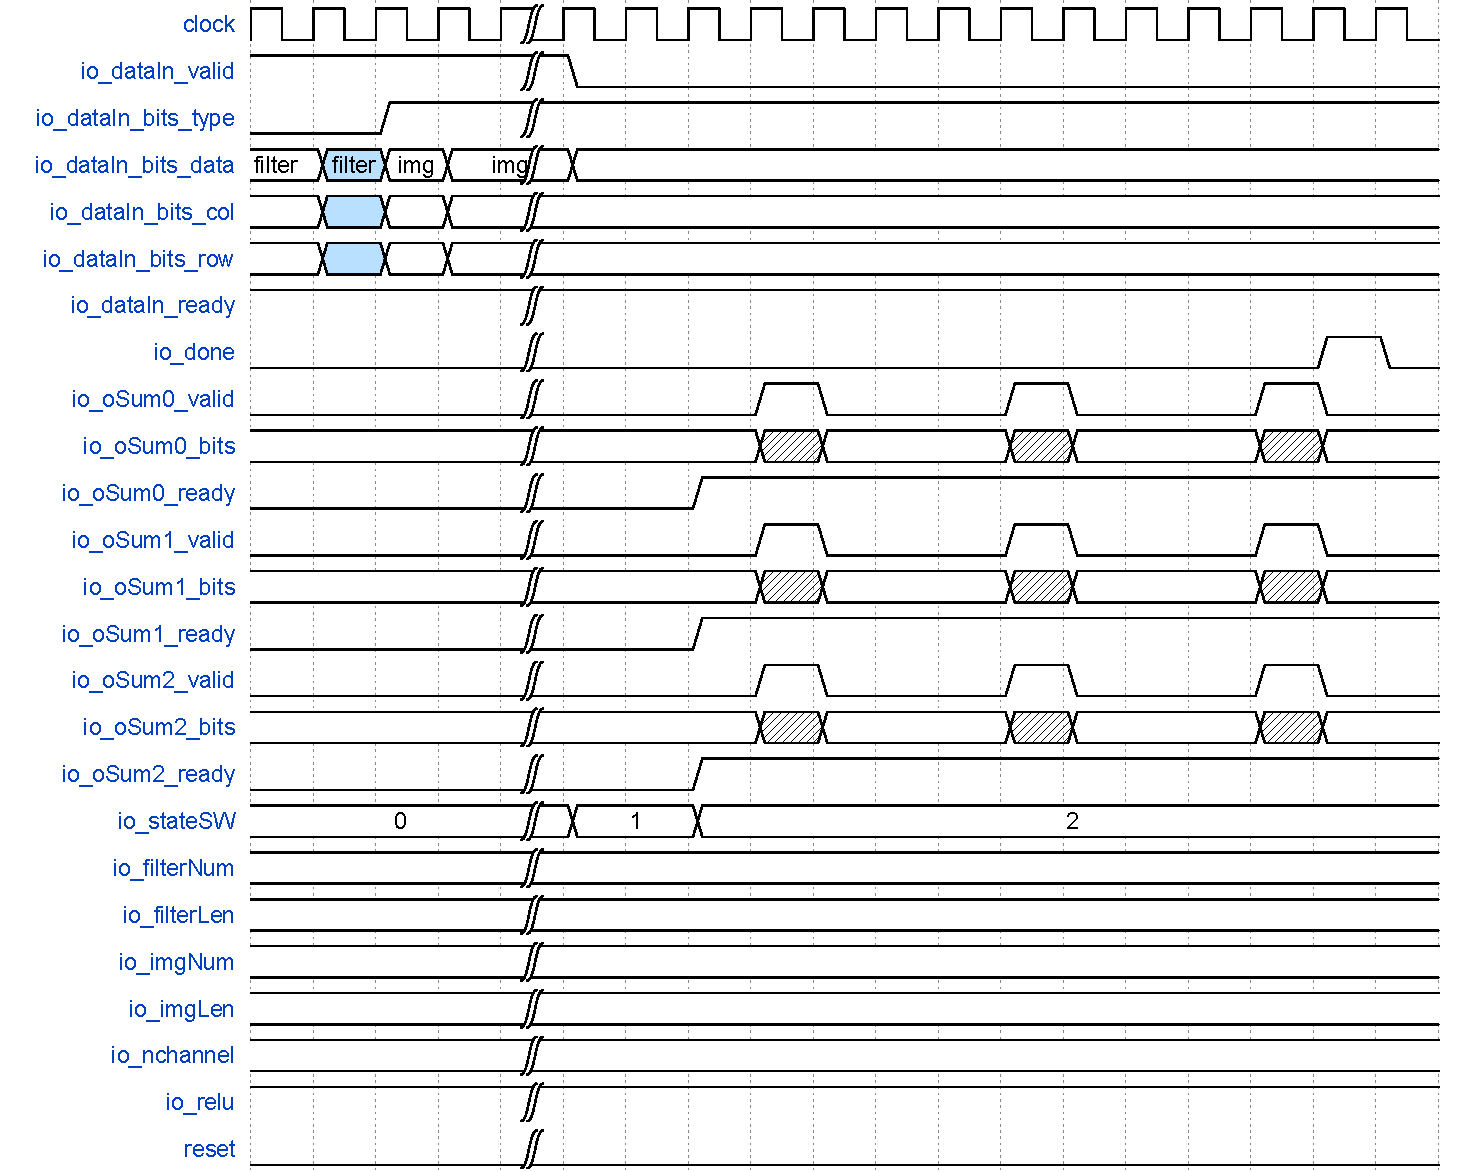
\includegraphics[scale=0.65]{../pdf/pearray_w.pdf}\\
    \caption{PEArray波形图}
\end{figure}
% [info] [0.405] filterNum: 3
% [info] [0.405] imgNum: 2
% [info] [0.405] channel: 3
% [info] [0.405] fLen: 3
% [info] [0.405] iLen: 5
% [info] [0.405] List(-3, -4, -3, -5, -3, 2, 1, -1, -4, -2, 2, -1, -1, 0, -2, -1, -4, -5, 4, -1, -4, -3, -5, -5, 1, 4, -3)
% [info] [0.405] 
% [info] [0.405] List(4, 0, 3, -4, 3, 4, -3, 2, 0, 4, 1, 0, -1, 1, 4, 0, 0, -3, 1, 1, -5, 1, 2, -5, -3, -4, -3)
% [info] [0.405] 
% [info] [0.405] List(3, 4, -4, 1, 1, 4, -3, -1, 1, 1, -4, -3, -4, -2, -3, 4, -4, -3, 3, -4, -4, 1, -2, 3, -4, 4, 1)
% [info] [0.405] 
% [info] [0.405] img2d: 
% [info] [0.406] List(3, 0, -4, -5, -2, 1, 2, 2, -2, 0, 2, -1, -4, 0, 2, -1, 2, 0, 2, -4, -1, 1, -4, 2, -3, 4, 2, 3, 1, 0)
% [info] [0.406] 
% [info] [0.406] List(-5, -5, 4, 1, -4, -2, 0, 4, -2, -3, 0, -2, 0, -2, 2, -2, 3, 0, 2, 0, 1, 1, -5, -2, 4, -4, 0, -2, -4, -5)
% [info] [0.406] 
% [info] [0.406] List(-1, 0, -4, -2, 2, 3, 0, 4, 2, -1, 4, -5, 0, 3, -1, 0, 0, 0, 4, 2, 2, -4, -2, -5, 2, 3, -4, 1, 3, 2)
% [info] [0.406] 
% [info] [0.406] List(2, 2, 1, 2, -1, 0, -4, -3, -5, 3, -3, 1, 4, 0, 2, -5, 1, -2, 0, -2, 1, 2, 0, -3, -1, 1, 2, 4, 2, -2)
% [info] [0.406] 
% [info] [0.406] List(4, -5, 2, 3, 1, -4, -1, -5, 4, 1, 4, 0, -3, -4, -2, -4, 1, -2, -2, 0, 4, 0, 3, -4, 1, -5, 4, 4, -3, -4)
% [info] [0.406] 
% [info] [0.406] sw: 
% [info] [0.407] 11  40  0  
% 46  0   0  
% 0   32  0  
% [info] [0.407] 
% [info] [0.408] 0   0    5  
% 10  103  7  
% 40  0    0  
% [info] [0.408] 
% [info] [0.408] 0  46  75  
% 0  33  50  
% 0  0   0   
% [info] [0.408] 
% [info] [0.408] 12  22  60   
% 48  8   65   
% 0   0   112  
% [info] [0.408] 
% [info] [0.408] 15  10  0   
% 0   56  0   
% 0   0   20  
% [info] [0.408] 
% [info] [0.408] 38  0   0  
% 93  32  0  
% 17  1   0  
% [info] [0.408] 
% [info] [0.576] jj reduce: 54
% [info] [0.576] sw1d: 54
% [info] [0.583] loop: 1
% [info] [0.583] ===============ERROR: 0======================


\section{运行MNIST测试结果}
    \subsection{模型量化}
    \subsection{运行流程}
    \subsection{输出结果与数学结果映射关系}

\section{系统性能}
    \subsection{资源占用}
    使用Chisel3 MEM:
    \begin{figure}[h]
        \centering
        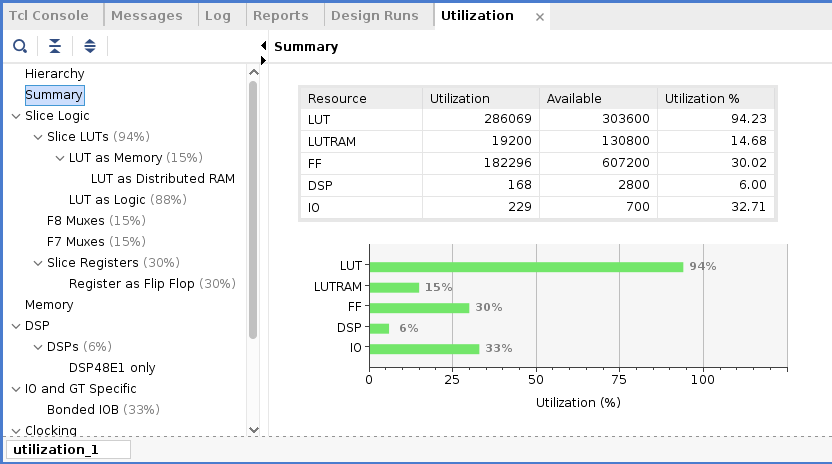
\includegraphics[scale=0.5]{../pdf/old_resource.png}\\
        \caption{使用MEM的资源报告}
    \end{figure}
    使用DW ip优化之后:
    \begin{figure}[h]
        \centering
        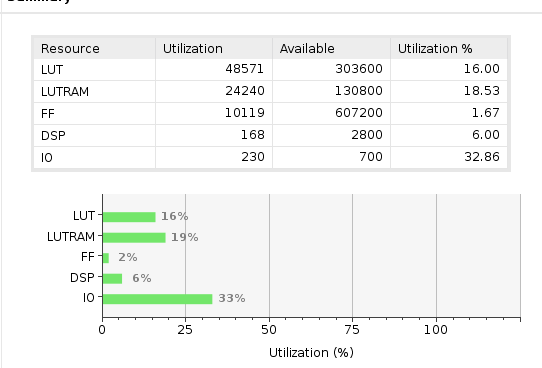
\includegraphics[scale=0.5]{../pdf/new_resource.png}\\
        \caption{使用DW ip的资源报告}
    \end{figure}

    \subsection{时序报告}
    使用Chisel3 MEM:
    \begin{figure}[h]
        \centering
        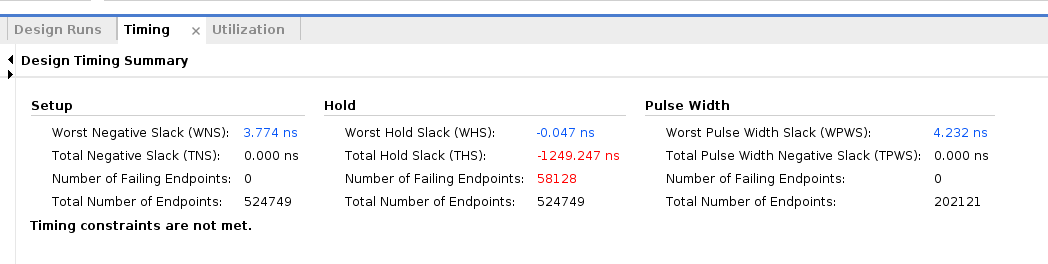
\includegraphics[scale=0.4]{../pdf/old_time.png}\\
        \caption{使用MEM的时序报告}
    \end{figure}
    使用DW ip优化之后:
    \begin{figure}[h]
        \centering
        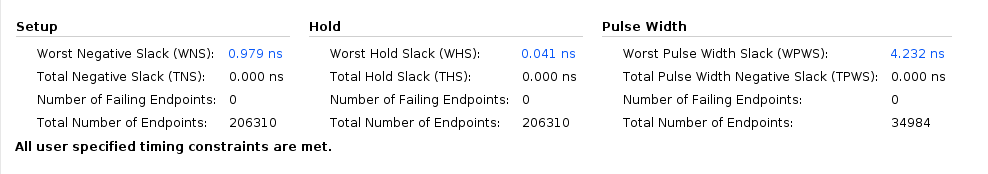
\includegraphics[scale=0.4]{../pdf/new_time.png}\\
        \caption{使用DW ip的时序报告}
    \end{figure}

\section{本章小结}
% \subsection{二级节标题}

% \subsubsection{三级节标题}

% \paragraph{四级节标题}

% \subparagraph{五级节标题}

% \section{脚注}

% Lorem ipsum dolor sit amet, consectetur adipiscing elit, sed do eiusmod tempor
% incididunt ut labore et dolore magna aliqua. Ut enim ad minim veniam, quis
% nostrud exercitation ullamco laboris nisi ut aliquip ex ea commodo consequat.
% Duis aute irure dolor in reprehenderit in voluptate velit esse cillum dolore eu
% fugiat nulla pariatur. Excepteur sint occaecat cupidatat non proident, sunt in
% culpa qui officia deserunt mollit anim id est laborum.
% \footnote{This is a long long long long long long long long long long long long
% long long long long long long long long long long footnote.}
